\begin{problem}[问题6.9]
设一蒙古包是一半径为$a$的半圆球形, 受到速度为$V_\infty$的大风袭击, 屋顶
承受一向上的升力, 有掀翻蒙古包的危险. 假设蒙古包内的压强为流体
的驻点压强, 求蒙古包受到的拔力.(假设流动为理想不可压缩无旋流)
\end{problem}
\begin{solution}
\begin{multicols}{2}
\noindent\textbf{解:} 建立如图\ref{fig:halfsphere}所示的极坐标系. 由轴对称无旋流动的圆球绕流结论知, 速度势为
\[
\varphi = v_\infty r\Big(1+\frac{a^3}{2r^3}\Big)\cos\theta
\]
因此有
\[
v_r = \frac{\partial \varphi}{\partial r} = v_\infty\Big(1-\frac{a^3}{r^3}\Big)\cos\theta
\]
\[
v_\theta = \frac{\partial \varphi}{r\partial\theta} =
-v_\infty r\Big(1+\frac{a^3}{2r^3}\Big)\sin\theta
\]
对于蒙古包表面有$r=a$, 因此蒙古包表面
\[
u_r = 0, {~} u_\theta = -\frac{3}{2}v_\infty\sin\theta
\]

\begin{center}
%\includegraphics[width=0.4\textwidth]{./figures/p9.pdf}

\usetikzlibrary{calc,fadings,decorations.pathreplacing}

\newcommand\pgfmathsinandcos[3]{%
  \pgfmathsetmacro#1{sin(#3)}%
  \pgfmathsetmacro#2{cos(#3)}%
}
\newcommand\LongitudePlane[3][current plane]{%
  \pgfmathsinandcos\sinEl\cosEl{#2} % elevation
  \pgfmathsinandcos\sint\cost{#3} % azimuth
  \tikzset{#1/.style={cm={\cost,\sint*\sinEl,0,\cosEl,(0,0)}}}
}
\newcommand\LatitudePlane[3][current plane]{%
  \pgfmathsinandcos\sinEl\cosEl{#2} % elevation
  \pgfmathsinandcos\sint\cost{#3} % latitude
  \pgfmathsetmacro\yshift{\cosEl*\sint}
  \tikzset{#1/.style={cm={\cost,0,0,\cost*\sinEl,(0,\yshift)}}} %
}
\newcommand\DrawLongitudeCircle[2][1]{
  \LongitudePlane{\angEl}{#2}
  \tikzset{current plane/.prefix style={scale=#1}}
   % angle of "visibility"
  \pgfmathsetmacro\angVis{atan(sin(#2)*cos(\angEl)/sin(\angEl))} %
  \draw[current plane] (\angVis:1) arc (\angVis:\angVis+180:1);
  \draw[current plane,dashed] (\angVis-180:1) arc (\angVis-180:\angVis:1);
}
\newcommand\DrawLatitudeCircle[2][1]{
  \LatitudePlane{\angEl}{#2}
  \tikzset{current plane/.prefix style={scale=#1}}
  \pgfmathsetmacro\sinVis{sin(#2)/cos(#2)*sin(\angEl)/cos(\angEl)}
  % angle of "visibility"
  \pgfmathsetmacro\angVis{asin(min(1,max(\sinVis,-1)))}
  \draw[current plane,black!60] (\angVis:1) arc (\angVis:-\angVis-180:1);
  \draw[current plane,dashed,black!60] (180-\angVis:1) arc (180-\angVis:\angVis:1);
}

%% document-wide tikz options and styles

\tikzset{%
  >=latex, % option for nice arrows
  inner sep=0pt,%
  outer sep=2pt,%
  mark coordinate/.style={inner sep=0pt,outer sep=0pt,minimum size=3pt,
    fill=black,circle}%
}



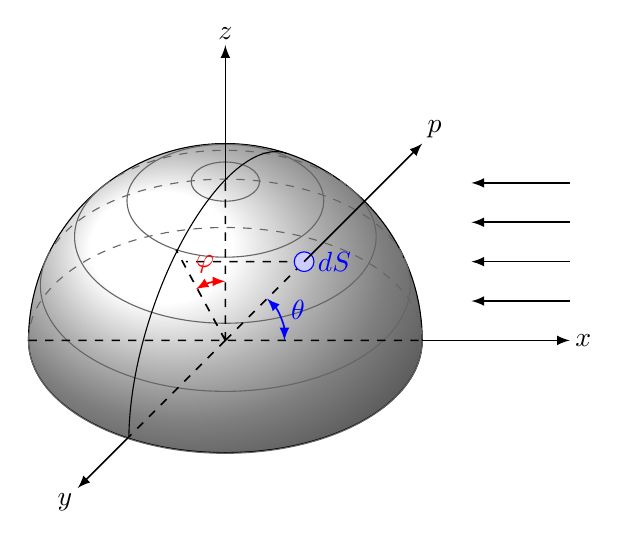
\begin{tikzpicture} % "THE GLOBE" showcase

\def\R{2.5} % sphere radius
\def\angEl{35} % elevation angle
\filldraw[ball color=white] (\R,0) arc (0:180:\R) arc(180:360:{\R} and 0.57*\R);
\foreach \t in {0,20,...,80} { \DrawLatitudeCircle[\R]{\t} }
%\foreach \t in {-120} { \DrawLongitudeCircle[\R]{\t} }
\draw[rotate=-18](0,\R) arc(90:218:{0.4*\R} and \R);
\draw[semithick,dashed](-\R,0)--(\R,0) (0,0)--(0,0.8*\R) (0,0)--(-0.5*\R,-0.5*\R) (0,0)--(0.4*\R,0.4*\R) (0.4*\R,0.4*\R)--(-0.2*\R,0.4*\R) (0,0)--(-0.25*\R,0.46*\R);
 %(0,0)--(-0.385*\R,0.1475*\R)--(0.39*\R,0.15*\R)--(0,0);
\draw[semithick,->] (\R,0)--(1.75*\R,0) node[right]{$x$};
\draw[semithick,->] (0,0.8*\R)--(0,1.5*\R) node[above]{$z$};
\draw[semithick,->] (-0.5*\R,-0.5*\R)--(-0.75*\R,-0.75*\R) node[below left]{$y$};

\fill[blue!20,draw=blue](0.4*\R,0.4*\R) circle(0.125) node[right=3pt,blue]{$dS$};
\draw[semithick,->] (0.4*\R,0.4*\R)--(\R,\R) node[above right]{$p$};
\draw[<->,semithick,blue] (0:0.75) arc(0:45:0.75);

\draw[<->,semithick,red] (90:0.75) arc(90:120:0.75);
\node[red] at (105:1){$\varphi$};

\node[blue] at (22.5:1) {$\theta$};


\draw[semithick,->] (1.75*\R,0.5)--(1.25*\R,0.5);
\draw[semithick,->] (1.75*\R,1)--(1.25*\R,1);
\draw[semithick,->] (1.75*\R,1.5)--(1.25*\R,1.5);
\draw[semithick,->] (1.75*\R,2.0)--(1.25*\R,2.0);

%\draw

\end{tikzpicture}
\captionof{figure}{蒙古包的极坐标系示意图}\label{fig:halfsphere}
\end{center}
\end{multicols}
\noindent 又由伯努力方程
\[
\frac{v_\infty^2}{2} + \frac{p_\infty}{\rho} = \frac{v_\theta^2}{2} + \frac{p_\theta}{\rho} \Longrightarrow p_\theta = p_\infty + \frac{\rho}{2}v_\infty^2\Big(1-\frac{9}{4}\sin^2\theta\Big)
\]
驻点压强为$p_\infty + \rho v_\infty^2/2$. 因此作用在蒙古包内外压强差
\[
p = p_\infty + \frac{\rho}{2} v_\infty^2 - p_\theta = \frac{9}{8}\rho v_\infty^2\sin^2\theta
\]
设蒙古包曲面为$S$, 则半球面(蒙古包)上的面积元$dS = a^2\sin\theta d\theta d\varphi$. 因此蒙古包受到的拔力为
\begin{eqnarray}
F_z &=& \iint p\sin\theta\sin\varphi dS\nonumber\\
    &=& \frac{9}{8}a^2\rho v_\infty^2\int_0^{\pi}\sin\varphi d\varphi  \int_0^{\pi}\sin^4\theta d\theta\nonumber\\
    &=& \frac{27}{32}\pi a^2 \rho v_\infty^2\nonumber
\end{eqnarray}
\end{solution} 
